\pgfplotsset{compat=1.5}
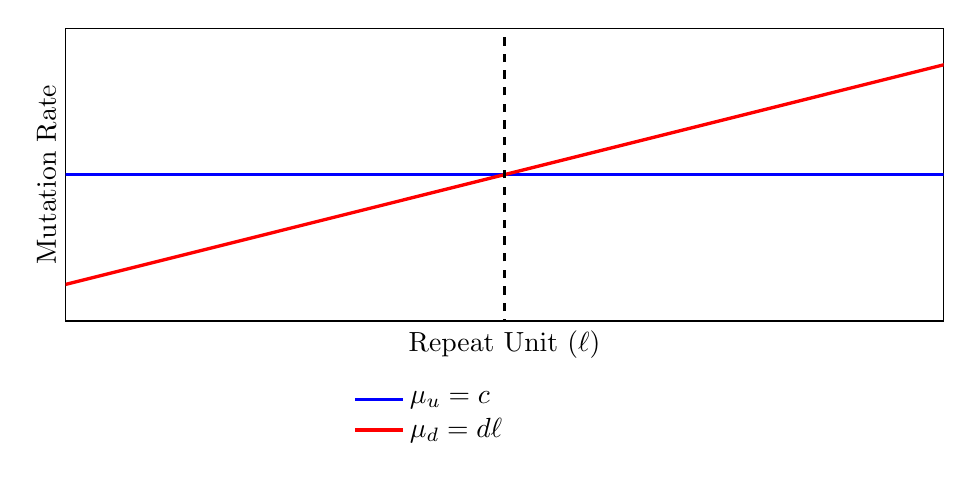
\begin{tikzpicture}
    \begin{axis}[
    width=1.05\linewidth, height=5.3cm,
    ylabel={Mutation Rate}, ymin=0.01, ymax=0.05,
    xlabel={Repeat Unit ($\ell$)}, xmin=6, xmax=18,
    xtick={0, 2, 4, 6, 8, 10, 12, 14, 16, 18, 20, 22, 24},
    samples=100, no markers, enlargelimits=false, legend style={at={(0.5,-0.2)},anchor=north,draw=none},
    legend cell align={left}, domain=0:25, ticks=none
    ]
        \addplot+[very thick]{0.03};
        \addlegendentry{$\mu_u = c$};

        \addplot+[very thick] {0.0025*x};
        \addlegendentry{\vspace*{5em}$\mu_d = d\ell$ \hspace*{5em}};

        \addplot+[very thick, black, dashed, forget plot] coordinates {(12, 0) (12, 0.05)};
    \end{axis}
\end{tikzpicture}